\label{sec_penalty}

\index{penalty formulation}

In order to impose the incompressibility constraint, two widely used procedures are available, namely the 
Lagrange multiplier method and the penalty method \cite{bathe82,hugh}. The latter is implemented in {\sc elefant}, which allows for the elimination of the pressure variable from the momentum equation (resulting in a reduction of the matrix size).%, based on a relaxation of the incompressibility constraint. 

Mathematical details on the origin and validity of the penalty approach applied to the Stokes problem can for instance be found in  \cite{cuss86}, \cite{redd82} or \cite{gunz89}.

The penalty formulation of the mass conservation equation is based on a relaxation of the incompressibility constraint and writes 
\begin{equation}
{\vec \nabla}\cdot {\vec \upnu} + \frac{p}{\lambda} = 0 \label{penal}
\end{equation}
where $\lambda$ is the penalty parameter, that can be interpreted (and has the same dimension) as a bulk viscosity. It is 
equivalent to say that the material is weakly compressible. It can be shown that if one chooses $\lambda$ to be a 
sufficiently large number, the continuity equation $ {\vec \nabla}\cdot {\vec \upnu} = 0$ will be approximately satisfied in the finite element solution. The value of $\lambda$ is often recommended to be 6 to 7 orders of magnitude larger than the shear viscosity \cite{dohu03,hulb79}.

%Note that Eq. (\ref{penal}) does not form the basis of the penalty method (as often implied) for the Stokes equation but is a consequence of minimising a modified functional of the problem under certain assumptions \cite{redd82}. 

Equation (\ref{penal}) can be used to eliminate the pressure in Eq. (\ref{mce2}) so that the mass and momentum conservation equations fuse to become :
\begin{equation}
{\vec \nabla}\cdot ( 2 \eta \dot\varepsilon({\vec \upnu})) 
+ \lambda {\vec \nabla} ({\vec \nabla }\cdot {\vec \upnu}) = \rho {\bm g} = 0 \label{peneq}
\end{equation}

\cite{mahu78} have established the equivalence for incompressible problems between the reduced integration
of the penalty term and a mixed Finite Element approach if the pressure nodes coincide with the integration points of the reduced rule.

In the end, the elimination of the pressure unknown in the Stokes equations
replaces the original saddle-point Stokes problem \cite{begl05} by an elliptical problem, 
which leads to a symmetric positive definite (SPD) FEM matrix. 
%Such systems always admit a square root triangular matrix (the Cholesky factor, L) and can be solved, once L has been computed (Cholesky factorization), by 2 triangular matrix solves (upper and lower back-substitutions). 
This is the major benefit of the penalized approach 
over the full indefinite solver with the velocity-pressure variables. Indeed, the SPD character of the matrix lends itself 
to efficient solving stragegies and is less memory-demanding since it is sufficient to store only the upper half of the matrix including the diagonal
\cite{gova}
.
\improvement{list codes which use this approach}

The stress tensor ${\bm \sigma}$ is symmetric ({\it i.e.} $\sigma_{ij}=\sigma_{ji}$). For simplicity
I will now focus on a Stokes flow in two dimensions. 

Since the penalty formulation is only valid for incompressible flows, then 
$\dot{\bm \epsilon}=\dot{\bm \epsilon}^d$ so that the $d$ superscript is ommitted in what follows.
The stress tensor can also be cast in vector format:
\begin{eqnarray}
\left(
\begin{array}{c}
\sigma_{xx}\\
\sigma_{yy}\\
\sigma_{xy}\\
\end{array}
\right)
&=&
\left(
\begin{array}{c}
-p \\
-p\\
0
\end{array}
\right)
+2 \eta
\left(
\begin{array}{c}
\dot{\epsilon}_{xx}\\
\dot{\epsilon}_{yy}\\
\dot{\epsilon}_{xy}\\
\end{array}
\right)
\nonumber\\
&=&
\lambda
\left(
\begin{array}{c}
\dot{\epsilon}_{xx} + \dot{\epsilon}_{yy}\\
\dot{\epsilon}_{xx} + \dot{\epsilon}_{yy}\\
0
\end{array}
\right)
+2 \eta
\left(
\begin{array}{c}
\dot{\epsilon}_{xx}\\
\dot{\epsilon}_{yy}\\
\dot{\epsilon}_{xy}\\
\end{array}
\right)\nonumber\\
&=&
\left[
\lambda
\underbrace{
\left(
\begin{array}{ccc}
1 & 1 & 0\\
1 & 1 & 0\\
0 & 0 & 0\\
\end{array}
\right)}_{\bm K}
+ \eta
\underbrace{
\left(
\begin{array}{ccc}
2 & 0 & 0 \\
0 & 2 & 0 \\
0 & 0 & 1 \\
\end{array}
\right)
}_{\bm C}
\right]
\cdot
\left(
\begin{array}{c}
\frac{\partial u}{\partial x} \\ \\
\frac{\partial v}{\partial y} \\ \\
\frac{\partial u}{\partial y} + \frac{\partial v}{\partial x} \\
\end{array}
\right) \nonumber
\end{eqnarray}


Remember that
\[
\frac{\partial u}{\partial x} = \sum_{i=1}^4 \frac{\partial N_i}{\partial x}\;  u_i 
\quad\quad
\frac{\partial v}{\partial y} = \sum_{i=1}^4 \frac{\partial N_i}{\partial y}\;  v_i 
\]

\[
\frac{\partial u}{\partial y} 
+\frac{\partial v}{\partial x} 
= \sum_{i=1}^4 \frac{\partial N_i}{\partial y}\;  u_i
+ \sum_{i=1}^4 \frac{\partial N_i}{\partial x}\;  v_i
\]

so that
\[
\left(
\begin{array}{c}
\frac{\partial u}{\partial x} \\ \\
\frac{\partial v}{\partial y} \\ \\
\frac{\partial u}{\partial y} + \frac{\partial v}{\partial x} \\
\end{array}
\right)
=
\underbrace{
\left(
\begin{array}{cccccccc}
\frac{\partial N_1}{\partial x} & 0 & \frac{\partial N_2}{\partial x} & 0 & \frac{\partial N_3}{\partial x} & 0 & \frac{\partial N_4}{\partial x} & 0 \\  \\
0 & \frac{\partial N_1}{\partial y} & 0 & \frac{\partial N_2}{\partial y} & 0 & \frac{\partial N_3}{\partial y} & 0 & \frac{\partial N_4}{\partial y}  \\ \\
\frac{\partial N_1}{\partial y} &  \frac{\partial N_1}{\partial x} &  \frac{\partial N_2}{\partial y} &  \frac{\partial N_2}{\partial x} & 
\frac{\partial N_3}{\partial y} &  \frac{\partial N_3}{\partial x} &  \frac{\partial N_3}{\partial y} &  \frac{\partial N_4}{\partial x}  
\end{array}
\right)
}_{\bm B}
\cdot
\underbrace{
\left(
\begin{array}{c}
u1 \\ v1 \\ u2 \\ v2 \\ u3 \\ v3 \\ u4 \\ v4
\end{array}
\right)
}_{\bm V}
\]
Finally,
\[
\vec{\sigma}=
\left(
\begin{array}{c}
\sigma_{xx}\\
\sigma_{yy}\\
\sigma_{xy}\\
\end{array}
\right)
=
(\lambda {\bm K} +  \eta {\bm C} )\cdot {\bm B} \cdot {\bm V}
\]

\index{weak form}
We will now establish the weak form of the momentum conservation equation. 
We start again from 
\[
{\vec \nabla}\cdot {\bm \sigma} + {\vec b} = {\vec 0} 
\]
For the $N_i$'s 'regular enough', we can write:
\[
\int_{\Omega_e} N_i {\vec \nabla}\cdot {\bm \sigma} d\Omega + \int_{\Omega_e} N_i  {\bm b} d\Omega =0
\]
We can integrate by parts and drop the surface term\footnote{We will come back to this at a later stage}:
\[
\int_{\Omega_e} {\vec \nabla } N_i \cdot {\bm \sigma} d\Omega = \int_{\Omega_e} N_i  {\bm b} d\Omega 
\]
or, 
\[
\int_{\Omega_e} 
\left(
\begin{array}{ccc}
\frac{\partial N_i}{\partial x} & 0 & \frac{\partial N_i}{\partial y} \\  \\
0 & \frac{\partial N_i}{\partial y} &  \frac{\partial N_i}{\partial x}  
\end{array}
\right)
\cdot
\left(
\begin{array}{c}
\sigma_{xx}\\
\sigma_{yy}\\
\sigma_{xy}\\
\end{array}
\right)
d\Omega = \int_{\Omega_e} N_i {\bm b} d\Omega 
\]
Let $i=1,2,3,4$ and stack the resulting four equations on top of one another. 
\begin{eqnarray}
\int_{\Omega_e} 
\left(
\begin{array}{ccc}
\frac{\partial N_1}{\partial x} & 0 & \frac{\partial N_1}{\partial y} \\  \\
0 & \frac{\partial N_1}{\partial y} &  \frac{\partial N_1}{\partial x}  
\end{array}
\right)
\cdot
\left(
\begin{array}{c}
\sigma_{xx}\\
\sigma_{yy}\\
\sigma_{xy}\\
\end{array}
\right)
d\Omega &=& \int_{\Omega_e} N_1 
\left(
\begin{array}{c}
b_x \\ b_y
\end{array}
\right)
 d\Omega \\
\int_{\Omega_e} 
\left(
\begin{array}{ccc}
\frac{\partial N_2}{\partial x} & 0 & \frac{\partial N_2}{\partial y} \\  \\
0 & \frac{\partial N_2}{\partial y} &  \frac{\partial N_2}{\partial x}  
\end{array}
\right)
\cdot
\left(
\begin{array}{c}
\sigma_{xx}\\
\sigma_{yy}\\
\sigma_{xy}\\
\end{array}
\right)
d\Omega &=& \int_{\Omega_e} N_i 
\left(
\begin{array}{c}
b_x \\ b_y
\end{array}
\right)
d\Omega \\
\int_{\Omega_e} 
\left(
\begin{array}{ccc}
\frac{\partial N_3}{\partial x} & 0 & \frac{\partial N_3}{\partial y} \\  \\
0 & \frac{\partial N_3}{\partial y} &  \frac{\partial N_3}{\partial x}  
\end{array}
\right)
\cdot
\left(
\begin{array}{c}
\sigma_{xx}\\
\sigma_{yy}\\
\sigma_{xy}\\
\end{array}
\right)
d\Omega &=& \int_{\Omega_e} N_3 
\left(
\begin{array}{c}
b_x \\ b_y
\end{array}
\right)
d\Omega \\
\int_{\Omega_e} 
\left(
\begin{array}{ccc}
\frac{\partial N_4}{\partial x} & 0 & \frac{\partial N_4}{\partial y} \\  \\
0 & \frac{\partial N_4}{\partial y} &  \frac{\partial N_4}{\partial x}  
\end{array}
\right)
\cdot
\left(
\begin{array}{c}
\sigma_{xx}\\
\sigma_{yy}\\
\sigma_{xy}\\
\end{array}
\right)
d\Omega &=& \int_{\Omega_e} N_4 
\left(
\begin{array}{c}
b_x \\ b_y
\end{array}
\right)
d\Omega 
\end{eqnarray}
We easily recognize ${\bm B}^T$ inside the integrals!
Let us define 
\[
{\bm N}_b^T=(N_1 b_x , N_1 b_y, ... N_4 b_x, N_4 b_y)
\]
then we can write
\[
\int_{\Omega_e} {\bm B}^T \cdot 
\left(
\begin{array}{c}
\sigma_{xx}\\
\sigma_{yy}\\
\sigma_{xy}\\
\end{array}
\right)
d\Omega
=
\int_{\Omega_e} {\bm N}_b d\Omega 
\]
and finally:
\[
\int_{\Omega_e} {\bm B}^T \cdot [ \lambda {\bm K} + \eta {\bm C} ] \cdot {\bm B} \cdot {\bm V} d\Omega
=
\int_{\Omega_e} {\bm N}_b d\Omega 
\]
Since $V$ contains the velocities at the corners, it does not depend on the $x$ or $y$ coordinates
so it can be taking outside of the integral:
\[
\underbrace{
\left(\int_{\Omega_e} {\bm B}^T \cdot [ \lambda {\bm K} + \eta {\bm C} ] \cdot {\bm B} d\Omega \right) 
}_{A_{el}(8 \times 8)}
\cdot 
\underbrace{
{\bm V}
}_{(8x1)}
=
\underbrace{
\int_{\Omega_e} {\bm N}_b d\Omega 
}_{B_{el} (8\times 1)}
\]
or, 
\[
\left[
\underbrace{
\left(\int_{\Omega_e} \lambda {\bm B}^T \cdot {\bm K} \cdot {\bm B} d\Omega \right) 
}_{A_{el}^\lambda(8 \times 8)}
+
\underbrace{
\left(\int_{\Omega_e}  \eta {\bm B}^T \cdot {\bm C}  \cdot {\bm B} d\Omega \right) 
}_{A_{el}^\eta(8 \times 8)}
\right]
\cdot 
\underbrace{
{\bm V}
}_{(8x1)}
=
\underbrace{
\int_{\Omega_e} {\bm N}_b d\Omega 
}_{B_{el} (8\times 1)}
\]

INTEGRATION - MAPPING 

reduced integration \cite{hulb79}

\begin{enumerate}

\item partition domain $\Omega$ into elements $\Omega_e$, $e=1, ... n_{el}$.


\item loop over elements and for each element compute ${\bm A}_{el}$, ${\bm B}_{el}$ \\
\begin{center}
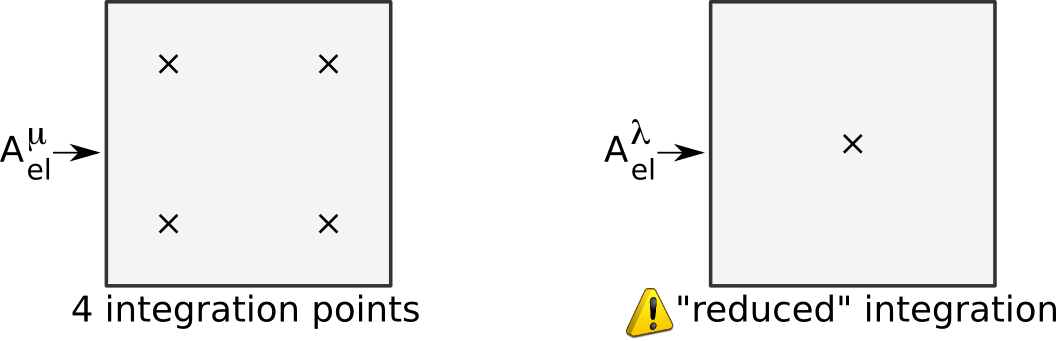
\includegraphics[width=5.5cm]{images/integration.png}
\end{center}

%
\includegraphics[width=0.5cm]{images/warning.png}
%4-point integration for ${\bm A}_{el}^\mu$, 1-point integration for ${\bm A}_{el}^\lambda$


\item a node belongs to several elements\\
      $\rightarrow$ need to assemble ${\bm A}_{el}$ and ${\bm B}_{el}$ in ${\bm A}$, ${\bm B}$

\item apply boundary conditions

\item solve system: ${\bm x}= {\bm A}^{-1} \cdot {\bm B}$
\item visualise/analyse ${\bm x}$
\end{enumerate}
